% "{'classe':('PSI'),'chapitre':'slci_p','type':('application'),'titre':'Réglage de correcteurs P', 'source':'CCMP MP 2010','comp':('C1-02','C2-04'),'corrige':True}"
%\setchapterimage{bandeau}
\chapter*{Application \arabic{cptApplication} \\ 
Réglage de correcteurs P -- 
\ifprof Corrigé \else Sujet \fi}
\addcontentsline{toc}{section}{Application \arabic{cptApplication} :
Réglage de correcteurs P -- 
\ifprof Corrigé \else Sujet \fi}

\iflivret \stepcounter{cptApplication} \else
\ifprof  \stepcounter{cptApplication} \else \fi
\fi

\setcounter{question}{0}
\marginnote{Etude d'un poste de palettisation de bidons. CCMP MP 2010.}
\marginnote[1cm]{
\UPSTIcompetence[2]{C1-02}
\UPSTIcompetence[2]{C2-04}}


La boucle de position est représentée figure ci-dessous. On admet que : 
\begin{itemize}
\item $H(p)=\dfrac{\Omega_m(p)}{U_v(p)}=\dfrac{K'_m}{1+\tau'_m p}=\dfrac{30}{1+5\cdot 10^{-3} p}$;
\item $K_r = \SI{4}{V.rad^{-1}}$ : gain du capteur de position;
\item $K_a$ : gain de l'adaptateur du signal de consigne $\alpha_e(t)$;
\item le signal de consigne $\alpha_e(t)$ est exprimé en degrés;
\item le correcteur $C(p)$ est à action proportionnelle de gain réglable $K_c$;
\item $N=200$ : rapport de transmission.
\end{itemize}

\begin{obj}
\begin{itemize}
\item On souhaite une marge de phase de 45\degres.
\item On souhaite un écart de traînage inférieur à 1\degres pour une consigne de vitesse de \SI{105}{\degres.s^{-1}}. 
\end{itemize}
\end{obj}

\begin{center}
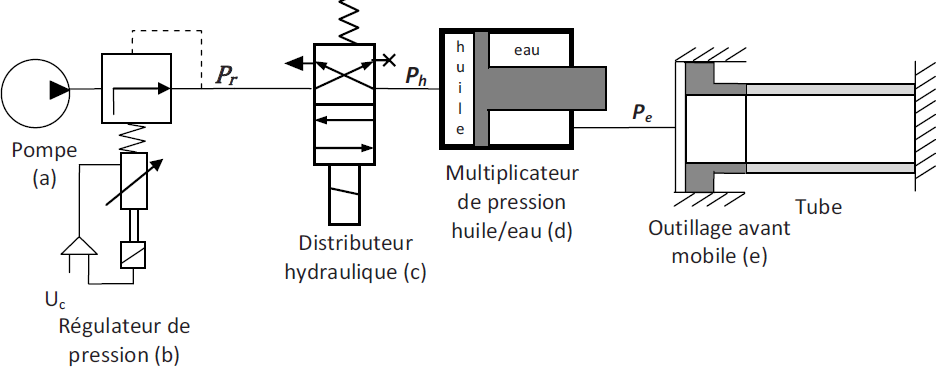
\includegraphics[width=\linewidth]{fig_01}
\end{center}

\question{Déterminer la fonctionde transfert $R(p)= \dfrac{\alpha_r(p)}{\Omega_m(p)}$ du réducteur.}
\ifprof
\begin{corrige}
D'une part le réducteur permet de réduire la vitesse. D'autre part, le schéma-bloc pemet de convertir une vitesse en position. Il joue donc le rôle d'intégrateur. On a donc $R(p)=\dfrac{1}{Np}$
\end{corrige}
\else
\fi


\question{Déterminer le gain $K_a$ de l'adaptateur.}
\ifprof
\begin{corrige}
On a 
$\varepsilon_(p)=K_a \alpha_e(p) - K_r \alpha_r(p) $
$=K_a \alpha_e(p) - K_r \dfrac{\pi}{180}\alpha_(p) $.
Pour que le système soit correctement asservi, il faut donc  $K_a =  K_r \dfrac{\pi}{180}$.
\end{corrige}
\else
\fi


\question{Déterminer, en fonction notamment de $K_m'$ et $t_m'$, la fonction de transfert
en boucle ouverte $T(p)$ que l’on exprimera sous forme canonique. En déduire l’expression du
gain de boucle, noté $K_{\text{BO}}$. }
\ifprof
\begin{corrige}
On a $T(p)= C(p)H(p)R(p)K_r$ 
$=K_c \dfrac{K'_m}{1+\tau'_m p}\dfrac{1}{Np} K_r  $. On a donc $\indice{K}{BO}=\dfrac{K_c K'_mK_r}{N} $
\end{corrige}
\else
\fi

On souhaite une marge de phase de 45\degres.

\question{Déterminer la valeur de $K_{\text{BO}}$ permettant de satisfaire cette condition.}
\ifprof
\begin{corrige}
Pour un premier ordre intégré, la phase est de 135\degres en $\dfrac{1}{\tau_m'}$. Le  gain (dB) de la boucle ouverte doit donc être nul pour cette pulsation ou encore que le module soit unitaire.

$|T(p)|=1$ 
$\Rightarrow \left| K_c \dfrac{K'_m}{1+\tau'_m p}\dfrac{1}{Np} K_r \right| = 1$ 
$\Rightarrow \dfrac{K_c K'_m K_r}{N} \left| \dfrac{1}{1+\tau'_m p}\dfrac{1}{p}  \right| = 1$ 
$\Rightarrow \dfrac{K_c K'_m K_r}{N\dfrac{1}{\tau_m'}}  \dfrac{1}{\sqrt{1+1 }}   = 1$ 
$\Rightarrow K_c   = \dfrac{N\sqrt{2}}{\tau_m' K'_m K_r}$ 
$\Rightarrow K_c   = \dfrac{\sqrt{2}}{\indice{K}{BO}}$ 

\end{corrige}
\else
\fi



\question{En déduire la valeur du gain $K_c$ du correcteur. }
\ifprof
\begin{corrige}
$\Rightarrow K_c   = \dfrac{N\sqrt{2}}{\tau_m' K'_m K_r}$ 
\end{corrige}
\else
\fi



\question{Déterminer l’écart de position. Conclure vis-à-vis des exigences du cahier des
charges. }
\ifprof
\begin{corrige}
La BO du sytème est de classe 1. Pour une entrée échelon, l'écart statique est nul. 
\end{corrige}
\else
\fi

On souhaite un écart de traînage inférieur à 1\degres~pour une consigne de vitesse de \SI{105}{\degres.s^{-1}}. 

\question{Déterminer l’expression de $\alpha_e(t)$ correspondant à une consigne de vitesse
de \SI{105}{\degres.s^{-1}}. En déduire $\alpha_e(p)$.}
\ifprof
\begin{corrige}
$\alpha_e(t) = 105 t$ et $\alpha_e(p)=\dfrac{105}{p^2}$
\end{corrige}
\else
\fi


\question{La valeur de $K_{\text{BO}}$ définie précédemment permet-elle de satisfaire l’exigence de précision imposée par le cahier des charges ? Conclure. }
\ifprof
\begin{corrige}
L'écart de trainage est donné par $\varepsilon_t = \dfrac{105 K_a}{\indice{K}{BO}}$
$= \dfrac{105 K_r \dfrac{\pi}{180} }{\dfrac{\dfrac{N\sqrt{2}}{\tau_m' K'_m K_r} K'_mK_r}{N}}$
$= \dfrac{105 \pi K_r\tau_m' }{180\sqrt{2}}$.

AN : $\varepsilon_t = \dfrac{105 \times  \pi \times 4 \times 5 \times 10^{-3} }{180\sqrt{2}} = 0,02\degres$. Le CDC est respecté. 
\end{corrige}
\else
\fi

\ifprof
\else
\begin{marginfigure}
\centering

\includegraphics[width=3cm]{Cy_03_01_Application_01_P_qr}
\end{marginfigure}
\fi



\ifprof
\else
\ifcolle
\else
\marginnote{
\begin{solution}
\begin{enumerate}
\item $R(p)=\dfrac{1}{Np}$.
\item $K_a = \dfrac{\pi}{180}K_r$.
\item $T(p)=\dfrac{K_{\text{BO}}}{p\left( 1+\tau'_m p\right)}$ avec $K_{\text{BO}}=\dfrac{K_cK'_m K_r}{N}$.
\item $K_{\text{BO}}=\dfrac{\sqrt{2}}{\tau'_m}$.
\item $K_c = \dfrac{\sqrt{2}N}{\tau'_m K'_M K_r}$.
\item $\varepsilon_S = 0$.
\item $\alpha_e (p) = \dfrac{105}{p^2}$.
\item $\varepsilon_d = \dfrac{105 K_a}{K_{\text{BO}}}$.
\end{enumerate}
\end{solution}}
\fi
\fi



